\documentclass[10pt]{beamer}
%\documentclass[10pt, handout]{beamer}
%\setbeameroption{show notes}

%\documentclass[10pt, a4paper]{article}
%\usepackage{beamerarticle}




\mode<article>{
	
	\usepackage{hyperref}
	
}
\mode<presentation>{
	
	\usetheme{Antibes}
	\usefonttheme{professionalfonts} 
	\usefonttheme{serif} % default family is serif
	
	%\usecolortheme{spruce} %зеленая, плохой цвет в заголовках 
	%\usecolortheme{albatross} %синяя, пхоло виден черный цвет
	
}

\newcommand{\MP}[1]{\mode<presentation>{#1} }
\newcommand{\MA}[1]{\mode<article>{#1} }

\newcommand{\ABS}[1]{\left| #1 \right|}
%\newcommand{\ABS}[1]{\mid #1 \mid}

\newcommand{\HREF}[2]{{\color{blue}\underline{\href{#1}{#2}}}}

\setbeamertemplate{caption}[numbered]


%\usepackage[T2A]{fontenc}
%\usepackage[utf8]{inputenc}
%\usepackage[russian]{babel}
%\usepackage{amsmath} %математические формулы



\usepackage{ifthen}

\usepackage{tikz}
\usetikzlibrary{arrows.meta}
\usetikzlibrary{calc}
\usetikzlibrary{decorations}
\usetikzlibrary{decorations.pathreplacing}
\newcommand{\rememb}[1]{\tikz[remember picture,baseline=-0.5ex]{\draw node[inner sep=0pt, outer sep=0pt] (#1){\strut};}}



\usepackage{fp}
\usepackage{tikz-3dplot}
\usepackage{environ}
\usepackage{animate}





\usepackage{xcolor}
%\usepackage[left=20mm,right=20mm,top=20mm,bottom=20mm,a4paper]{geometry} %поля

\usepackage{amsmath} %математические формулы
%\usepackage{amsfonts} %математические шрифты


\usepackage[e]{esvect}  %Красивая стрелочка вектора
%\let\oldvv\vv
\newcommand{\VV}[1]{\vv{#1\mathstrut}}



\usepackage{graphicx} %работа с каритнками


%\usepackage{multimedia}
%\usepackage{movie15}

%Для XeLatex/+
\usepackage{polyglossia}
\setdefaultlanguage{russian}
\setotherlanguage{english}
%\setkeys{russian}{babelshorthands=true} 


\usepackage{fontspec}

\setmainfont{Times New Roman} [Script=Cyrillic, Mapping=tex-text,]
\setsansfont{Arial} [Script=Cyrillic, Mapping=tex-text,]
%\setmonofont{Courier New} [Script=Cyrillic, Mapping=tex-text,]
\newfontfamily{\cyrillicfonttt}{Courier New}


%\usepackage{unicode-math}
%\setmathfont{TeX Gyre Termes Math}

%\setmainfont{CMU Serif}[Script=Cyrillic, Mapping=tex-text,]
%\setsansfont{CMU Sans Serif}[Script=Cyrillic, Mapping=tex-text,]
%\setmonofont{CMU Typewriter Text}[Script=Cyrillic, Mapping=tex-text,]


%-----------------


%\usepackage{caption}
%\DeclareCaptionLabelSeparator{dot}{~---~}            %Разделитель номер рисунка
%\captionsetup[figure]{justification=centering,labelsep=dot, format=plain}                        %Подпись рис. центр
%\captionsetup[table]{justification=raggedleft,labelsep=dot, format=plain, singlelinecheck=false} %Подпись табл. слева
%\captionsetup[lstlisting]{justification=raggedleft,labelsep=dot, format=plain, singlelinecheck=false}                     %Подпись рис. центр

\usepackage{indentfirst} %отступ первой строки


\usepackage[svgnames]{xcolor}


\usepackage{hyperref}

%\usepackage{showframe}


%\usepackage{tikz}

%\usepackage[hidelinks]{hyperref}%ссылки внутри документа \ref


\setlength\abovecaptionskip{-2pt}
%\setlength\belowcaptionskip{-14pt}

\setbeamerfont{caption}{size=\scriptsize}


\def\sectionname{Раздел}
\def\subsectionname{Подраздел}


\newcommand{\TC}[3]
{
	
	
	\begin{columns}
		\begin{column}{#1\textwidth}
			#2
		\end{column}
		\begin{column}{\fpeval{1-#1}\textwidth}
			#3
		\end{column}
	\end{columns}
}

\newcommand{\TCT}[3]
{
	
	\begin{columns}[T]
		\begin{column}{#1\textwidth}
			#2
		\end{column}
		\begin{column}{\fpeval{1-#1}\textwidth}
			#3
		\end{column}
	\end{columns}
}


\newcommand{\FRAME}[2]{
	\begin{frame}
		\frametitle{#1}
		#2
	\end{frame}
}

\newcommand{\FIG}[3]
{
	\begin{figure}
		\centering
		\includegraphics[width=#3]{#1}
		\caption{#2}
	\end{figure}
}

\newcommand{\vect}[1]{\overrightarrow{#1}}


\usepackage{qrcode}

\newcommand{\LECADDR}{https://clck.ru/3D3Efj}


\usepackage{newfile}

\edef\LectionNumber{0}
\edef\LectionTheme{0}

\let\oldsection\section
\let\oldsubsection\subsection


\AtBeginDocument
{
	\newoutputstream{CONTENT}
	\openoutputfile{\LectionNumber .gvr}{CONTENT}
	
	\expandafter\addtostream{CONTENT}{\noindent\textbf{\Large Лекция \LectionNumber~---~\LectionTheme}\unexpanded{\setcounter{SEC}{0}}\par}
}

\renewcommand{\section}[1]{
	\oldsection{#1}
	\expandafter\addtostream{CONTENT}{\noindent\hspace{2ex}\unexpanded{\hbox{\large\stepcounter{SEC}\theSEC ~ #1}}\par}
}

\renewcommand{\subsection}[1]{
	\oldsubsection{#1}
	\expandafter\addtostream{CONTENT}{\noindent\hspace{6ex}\unexpanded{\stepcounter{SUB}\theSUB ~ #1}\par}
}


%\renewcommand{\section}[1]{\MMM{#1}}

%\edef\subsection#1
{
	%\noexpand\subsection{#1}
	%
}


\newfontfamily\dnifamily[Scale = 0.795]{DniFont.TTF}

\newcommand{\dni}[1]{%
	{\dnifamily%
		\ifthenelse{#1=0}{0}{}%
		\ifthenelse{#1=1}{1}{}%
		\ifthenelse{#1=2}{2}{}%
		\ifthenelse{#1=3}{3}{}%
		\ifthenelse{#1=4}{4}{}%
		\ifthenelse{#1=5}{5}{}%
		\ifthenelse{#1=6}{6}{}%
		\ifthenelse{#1=7}{7}{}%
		\ifthenelse{#1=8}{8}{}%
		\ifthenelse{#1=9}{9}{}%
		\ifthenelse{#1=10}{)}{}%
		\ifthenelse{#1=11}{!}{}%
		\ifthenelse{#1=12}{@}{}%
		\ifthenelse{#1=13}{\#}{}%
		\ifthenelse{#1=14}{\$}{}%
		\ifthenelse{#1=15}{\%}{}%
		\ifthenelse{#1=16}{\^{}}{}%
		\ifthenelse{#1=17}{\&}{}%
		\ifthenelse{#1=18}{*}{}%
		\ifthenelse{#1=19}{(}{}%
		\ifthenelse{#1=20}{[}{}%
		\ifthenelse{#1=21}{]}{}%
		\ifthenelse{#1=22}{\textbackslash{}}{}%
		\ifthenelse{#1=23}{\{}{}%
		\ifthenelse{#1=24}{\}}{}%
		\ifthenelse{#1=25}{|}{}}%
}%

\newcommand{\toDni}[1]{%	
	\ifthenelse{#1=0}{}{%
		 \ifthenelse{#1=25}{%
		 	\expandafter\dni{#1}}{%
		 	\expandafter\toDni{\fpeval{floor(#1/25)}}%
		 \expandafter\dni{\fpeval{(#1/25 - floor(#1/25))/0.04}}}}%
}%



\newcommand{\Strut}{{\Large\strut}}

\newcommand\scb[1]{\left( #1 \right)}

\newcommand{\LINK}[2]{%
	\qrcode[height=1cm]{#1}\  \HREF{#1}{\parbox{0.8\textwidth}{#2}} \\[0.5em]
}

\NewDocumentCommand{\lecdni}{}{\toDni{\LectionNumber}}
\author{Гаврилов Андрей Геннадьевич}
\newcommand{\regals}{кандидат технических наук, доцент}
\institute{Кафедра Информационных технологий и вычислительных систем \\МГТУ~<<СТАНКИН>>}
\lecture{История компьютерной графики}{kghistory}\subtitle{Компьютерная графика}


\makeatletter
\newcommand*{\overlaynumber}{\number\beamer@slideinframe}
\makeatother



\usepackage{cprotect}

\newcommand{\QRFRAME}{%
    \begin{frame}[plain, noframenumbering]    	
	
	\centering
	Трансляция презентации (во время очных лекций)    
	
	~
	
	{\Large \ttfamily  https://clck.ru/3D3Efj  }
	
	~
	
	\tikz\node[inner sep=0pt,rounded corners=5mm, clip]{\qrcode[height=0.45\textwidth]{\LECADDR}}; 
	
	~	
	{\small
	При просмотре презентации в PDF для отображения анимаций на слайдах необходимо использовать Acrobat Reader, KDE Okular, PDF-XChange, Foxit Reader, браузер Firefox. Для браузеров на движке Chrome (Edge, Яндекс, Opera,~\dots) необходимо использовать \HREF{https://chromewebstore.google.com/detail/pdf-viewer/oemmndcbldboiebfnladdacbdfmadadm?hl=ru&utm_source=ext_sidebar}{PDF.js} c опцией <<Enable active content (JavaScript) in PDFs>>. }
	
	\end{frame}%
}

\newcommand{\IG}[2][1]{\includegraphics[width=#1\textwidth]{#2}}



\graphicspath{{Images/}{Images/\jobname/}}

\date{\today}

\renewcommand{\LectionNumber}{1}
\renewcommand{\LectionTheme}{История компьютерной графики}
\title{Лекция \lecdni \\ \LectionTheme}
\subtitle{Компьютерная графика}

\begin{document}
	 
		\makeatletter
\defbeamertemplate*{title page}{my theme}
{
	
	\hfill
	
	\begin{beamercolorbox}[wd=.9\paperwidth,center,]{title}%
		
	\end{beamercolorbox}%	
	
	\vbox to 1em {}
	
	\begin{beamercolorbox}[wd=.9\paperwidth,center,]{title}%
		\usebeamerfont{subtitle}%
		\hfill
		
		\insertsubtitle
		
		\usebeamerfont{title}%
		\inserttitle{} \\[0.5em]
		
		
		
	\end{beamercolorbox}%	
	\hfill\hfill
	
	\begin{beamercolorbox}[wd=.9\paperwidth,center,]{}%
		\usebeamerfont{author}%
		\hfill \\[0.5em]
		\insertauthor{} \\[0.5em]
		\regals
		    
		\vbox to 1em{}
		\usebeamerfont{institute}%
		\insertinstitute {}
		
		\vbox to 1em{}			
		{\; }\insertshortdate{}
		
	\end{beamercolorbox}%	
	\hfill\hfill
	
	\vbox to 5em{}
	
	
}
\defbeamertemplate*{footline}{my theme}{
	\leavevmode%
	\hbox{%
		\begin{beamercolorbox}[wd=.25\paperwidth,ht=3.25ex,dp=0ex,center,sep=1pt]{author in head/foot}%
			\usebeamerfont{author in head/foot}%
			\insertauthor 
			\beamer@ifempty{\insertshortinstitute}{}
		\end{beamercolorbox}%
		\begin{beamercolorbox}[wd=.65\paperwidth,ht=3.25ex,dp=0ex,center,sep=1pt]{title in head/foot}%
			\usebeamerfont{title in head/foot}\insertshortinstitute
		\end{beamercolorbox}%
		\begin{beamercolorbox}[wd=.1\paperwidth,ht=3.25ex,dp=0ex,center, sep=0.5pt]{date in head/foot}%
			\usebeamerfont{date in head/foot}
			\footnotesize \expandafter\toDni{\insertframenumber} / \expandafter\toDni{\inserttotalframenumber}
	\end{beamercolorbox}}%
}



\makeatother






%float page top aligment
\makeatletter
\setlength{\@fptop}{0pt}
\setlength{\@fpbot}{0pt plus 1fil}
\makeatother	 	
	
	\QRFRAME
	
	
	\frame{\maketitle}
	
	\begin{frame}\frametitle{План лекции}
		
		\tableofcontents
	\end{frame}
	
	\section{Структура курса}

	\begin{frame}
		\frametitle{Структура курса}
		\addcontentsline{toc}{subsection}{Первый фрейм} 
		
		\TCT{0.5}{
			
		
			\textbf{Первый семестр }
		
			
			
			\begin{itemize}
				\item 14 лекций
				\item 5 лабораторных работ  
				\item 4 семинара
				\item курсовая \emph{работа} 
				\item зачёт
			\end{itemize}
		
		}{
		
			\textbf{Второй семестр }
			
			\begin{itemize}
				\item 14 лекций
				\item 3 лабораторные работы  
				\item экзамен
			\end{itemize}
		
		
		}
		
		
	\end{frame}
	
	
	\section{История компьютерной графики}	
	
	
	\subsection {Предпосылки}
	
	\frame{\sectionpage}
	\frame{\subsectionpage}
	
	
	
	\begin{frame}
		\frametitle{Изобретение электронной лучевой трубки}

		\TC{0.5}{
			\begin{figure}
				\centering
				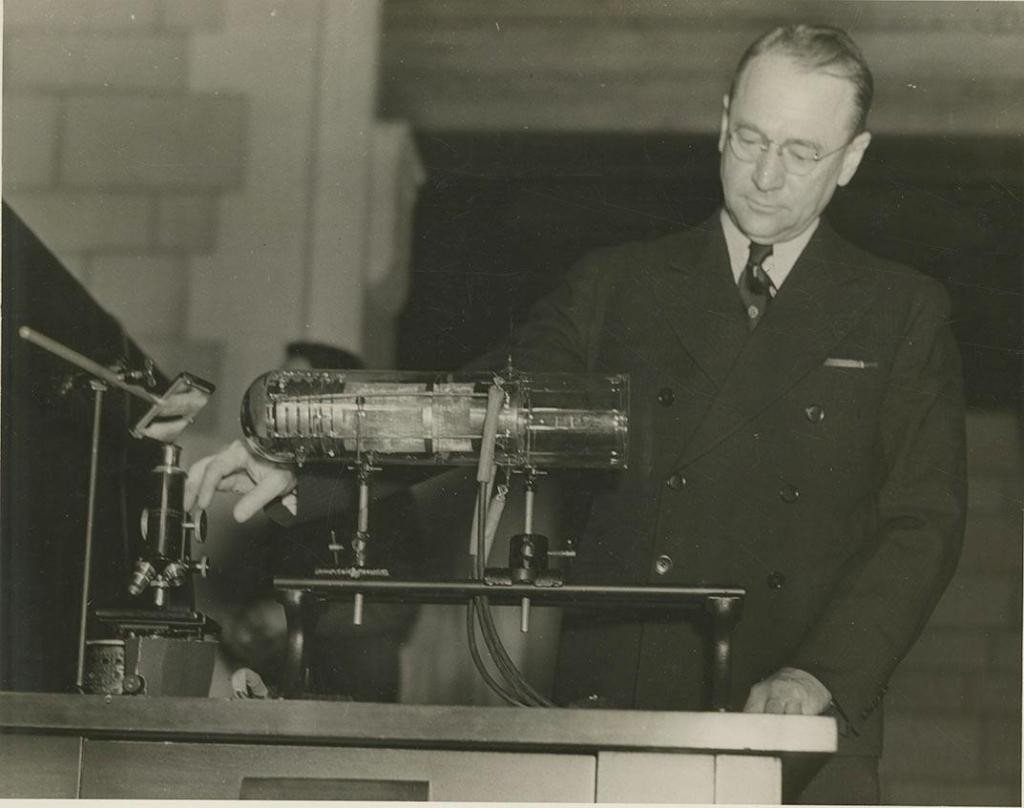
\includegraphics[width=1\textwidth]{10s3-full.jpg}
				\caption{Зворыкин К. З.}
			\end{figure}
		}{
		
		Владимир Козьмиич Зворыкин (29 июля 1888 года, Муром, Владимирская губерния, Российская империя — 29 июля 1982, Принстон, Нью-Джерси, США) 
		
		}		
		
	\end{frame}
	
	\begin{frame}
		\frametitle{Конструкция ЭЛТ}		

			\FIG{unnamed-1-750x542.jpg}{Принцип действия ЭЛТ}{0.7\textwidth}		
	\end{frame}
	
	
	\begin{frame}\frametitle{Рисунки на осцелографе}

		
		\TCT{0.4}{
			
			\begin{figure}
				\centering
				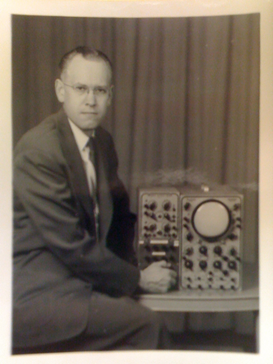
\includegraphics[width=1\textwidth]{Ben_F._Laposky.png}
				\caption{\centering Benjamin Francis Laposky (1914 – 2000) }
			\end{figure}
		
		}{
				В 1950 году Бенджамин Лапоски (Ben Laposky), математик, художник и чертежник, начал экспериментировать с рисованием на осциллографе.
		}
	\end{frame}
	
	\begin{frame}\frametitle{Рисунки на осцелографе}
	
		\begin{figure}
			\centering
			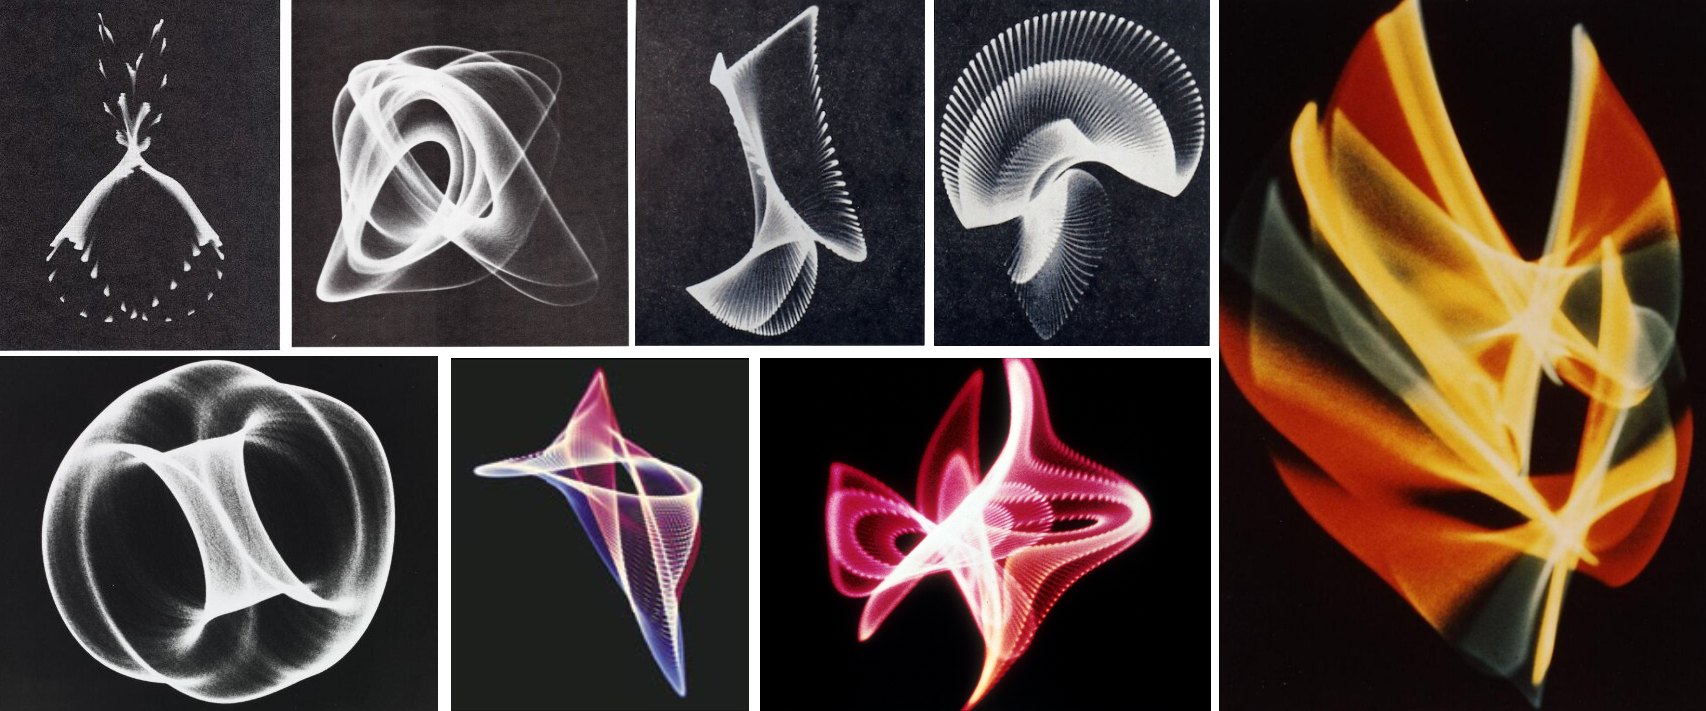
\includegraphics[width=1\textwidth]{osci.png}
			\caption{Работы Б. Лапосвки}
		\end{figure}

	\end{frame}
	
	\subsection{Первые динозвары}
	
	\frame{\subsectionpage}
	
	\begin{frame}\frametitle{Начало эры компьютерной графики}
	
		Декабрь 1951 года. В Массачусеттском технологическом институте (МТИ) для системы противовоздушной обороны военно-морского флота США был разработан первый дисплей для компьютера “Вихрь” (Whirlwind).		
		\begin{columns}[T]
			\begin{column}{0.5\textwidth}					
					\FIG{Museum_of_Science,_Boston,_MA_-_IMG_3168.JPG}{Whirlwind}{0.9\textwidth}	
			\end{column}
			\begin{column}{0.5\textwidth}
				\FIG{Jay_Forrester_1950s.jpg}{\centering Jay Wright Forrester (1918-2016)}{0.5\textwidth}
			\end{column}
		\end{columns}
		


	
	\end{frame}
	
\renewcommand\UrlFont{\color{red}\rmfamily\itshape}	

\begin{frame}\frametitle{Крестики-нолики}{
	OXO --- компьютерная игра для компьютера EDSAC. Разработана в 1952 году как иллюстрация диссертации на тему взаимодействия человека и компьютера.
	\begin{columns}[T]
		\begin{column}{0.33\textwidth}
			\begin{figure}
				\centering
				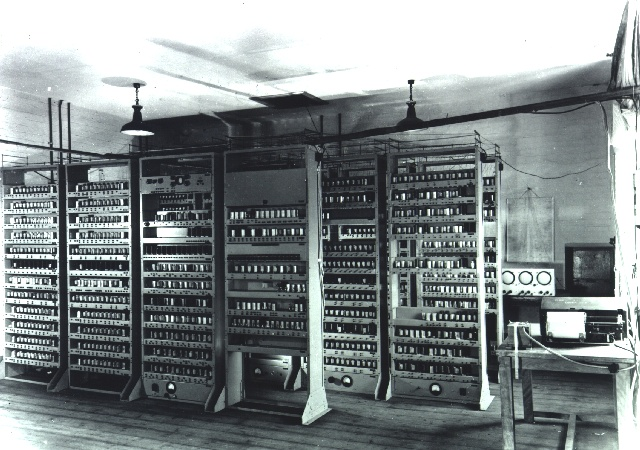
\includegraphics[width=1\textwidth]{EDSAC_(19).jpg}
				\caption{EDSAC}
			\end{figure}
		\end{column}
		\begin{column}{0.33\textwidth}
			\begin{figure}
			\centering
			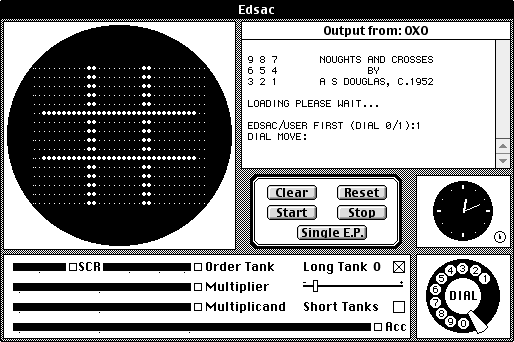
\includegraphics[width=1\textwidth]{OXO_emulated_screenshot.png}
			\caption{OXO}
			\end{figure}
		\end{column}
		\begin{column}{0.33\textwidth}
			\begin{figure}
			\centering
			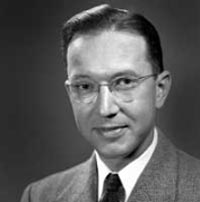
\includegraphics[width=0.8\textwidth]{alexander_douglas.jpg}
			\caption{\centering Alexander Shafto Douglas (1921–2010)}
			\end{figure}
		\end{column}
	\end{columns}
	
}\end{frame}

\begin{frame}\frametitle{Световое перо}{
	Световое перо было впервые создано в 1955 году в рамках проекта Whirlwind. 
    \begin{columns}[T]
    	\begin{column}{0.5\textwidth}
    		\begin{figure}
    			\centering
    			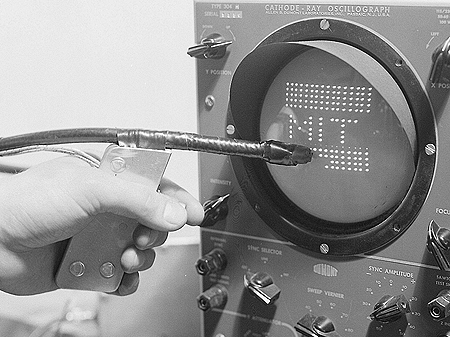
\includegraphics[width=1\textwidth]{light-pen-_ltpnmit.fit_lim.size_512x.png}
    			\caption{Прототип}
    		\end{figure}	
			
    	\end{column}
    	\begin{column}{0.5\textwidth}
    		\begin{figure}
    			\centering
    			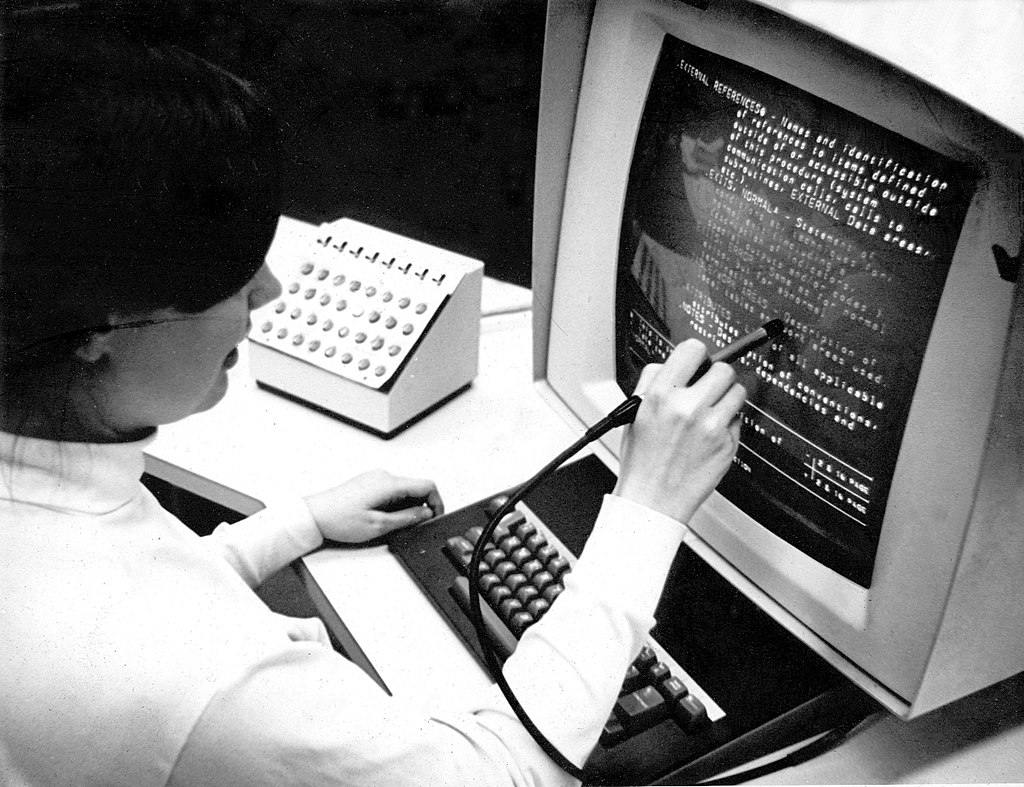
\includegraphics[width=1\textwidth]{HypertextEditingSystemConsoleBrownUniv1969.jpg}
    			\caption{Работа пера}
    		\end{figure}
    	\end{column}
    \end{columns}
}\end{frame}

\begin{frame}\frametitle{Первая цифровая фотография}
{
	\begin{columns}
		\begin{column}{0.4\textwidth}
			\begin{figure}
				\centering
				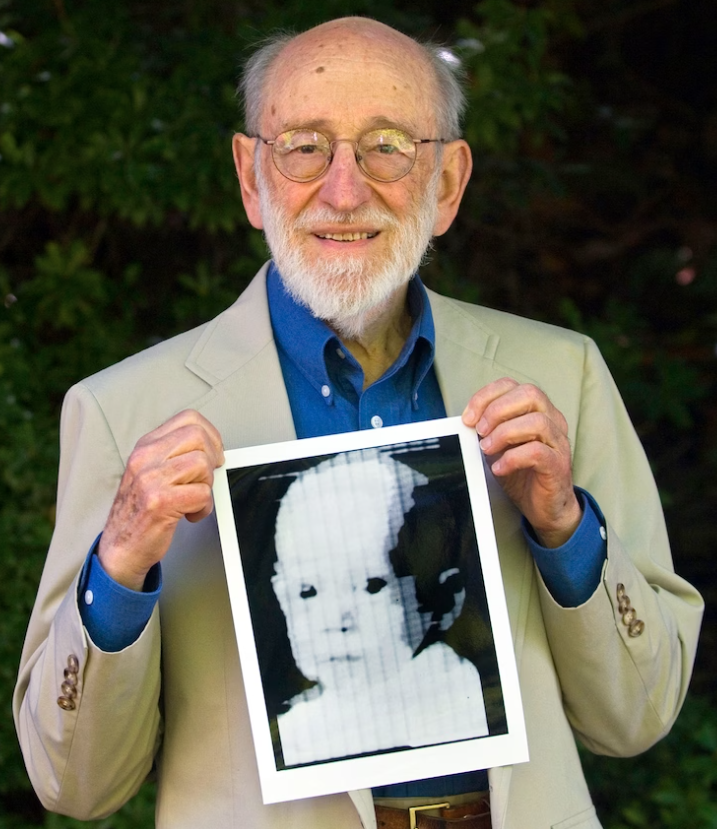
\includegraphics[width=1\textwidth]{Screenshot 2024-02-11 140345.png}
				\caption{\centering Рассел Кирш (1929-2020) }
			\end{figure}
		\end{column}
		\begin{column}{0.6\textwidth}
			В 1957 году группа Кирша разработала цифровой сканер изображений и выполнила первое цифровое сканирование.
			
			Пиксели, используемые для отображения фото и видео на экранах, были нововведением в 1957 году, тогда Кирш создал чёрно-белое цифровое изображение своего сына размером 2x2 дюйма.
		\end{column}
	\end{columns}
}\end{frame}

\begin{frame}\frametitle{Компьютерная графика}{

	\begin{columns}
		\begin{column}{0.6\textwidth}
			1960. Инженер-дизайнер Ульям Феттер  из авиастроительной корпорации Боинг впервые ввел термин <<Компьютерная графика>>. В 1964 году Ульям Феттер также создал на компьютере проволочную графическую модель человека и назвал её <<Человек Боинга>>
		\end{column}
		\begin{column}{0.4\textwidth}
				\begin{figure}
				\centering
				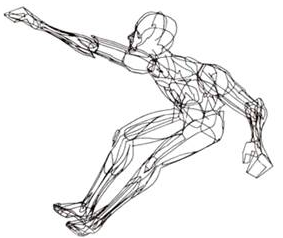
\includegraphics[width=1\textwidth]{Screenshot 2024-02-11 143003.png}
				\caption{\centering <<Человек Боинга>> }
			\end{figure}

		\end{column}
	\end{columns}

}\end{frame}

\begin{frame}\frametitle{Spacewar!}
{

	
		\begin{columns}
		\begin{column}{0.4\textwidth}
			\begin{figure}
			\centering
			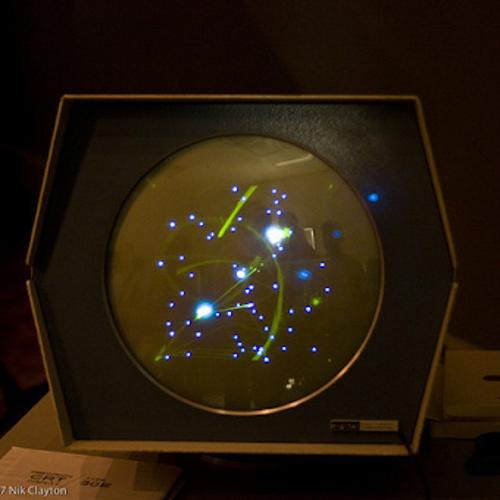
\includegraphics[width=1\textwidth]{1acdef914d2893a1ca8dbf4f1f8e5e03.jpg}
			\caption{Spacewar!}
		\end{figure}
		\end{column}
		\begin{column}{0.6\textwidth}
			Spacewar! — одна из первых известных цифровых компьютерных игр. Создана Стивом Расселом в 1962 году на платформе мини-компьютера DEC \HREF{https://ru.wikipedia.org/wiki/PDP-1}{PDP-1} в MIT. 
			
			\hfill
			
			\footnotesize \HREF{https://youtu.be/IoqA6fCyIpk?si=U1Zi1fYyxVrn2jax}{PDP-1 Demo at the CHM (short version)}
		\end{column}
	\end{columns}
	

}\end{frame}

	
	
\begin{frame}\frametitle{Sketchpad}{

\TC{0.5}{
			Айвен Сазерленд в 1962 году  создал  <<Блокнот>> (Sketchpad). Эта программа могла рисовать достаточно простые фигуры (точки, прямые, дуги окружностей), могла вращать фигуры на экране.
	
			\hfill
			
			\footnotesize \HREF{https://youtu.be/6orsmFndx_o?si=MArTbvP8qHzQ-g_l}{Ivan Sutherland Sketchpad Demo 1963}

}{
			\FIG{P91-233_RR_125218.jpg}{Ivan Sotherland (1938-н.в.)}{\textwidth}

}

}	\end{frame}


\begin{frame}\frametitle {DAC-1}
{
	\TC{0.4}{
		\FIG{2fab559cae06ac865760cb4c56a22eb5.jpg}{Терминал DAC-1}{\textwidth}
	}{В 1964 году General Motors представила систему автоматизированного проектирования DAC-1, разработанную совместно с IBM.
	
	\hfill
	
	\footnotesize \HREF {https://www.youtube.com/watch?v=Hasd8i8SFEg}{1964 DAC 1 early CAD system}
	}
	
	
}\end{frame}


\begin{frame}\frametitle {IBM 2250}
{
	\TC{0.4}
	{
		\FIG{Car-3D-Design-at-Mazda-in-1960s-1970s-with-IBM-2250-Model-3-System.jpg}{IBM 2250}{\textwidth}
	}
	{
		Графический дисплей IBM 2250 был анонсирован вместе с System / 360 в 1964 году. Полная система 2250 III с контроллером стоила около 280 000 долларов в 1970 году, хотя до 4 дисплеев могли использовать один контроллер, снижая стоимость отображения до 40
	}
	
}\end{frame}


\begin{frame}\frametitle {Poem Field}
{
	\TC{0.4}
	{
		\FIG{Screenshot 2024-02-12 164326.png}{Кадр из анимации}{\textwidth}
	}
	{
		В период 1965-1971 годов на основе BeFlix режиссером-экспериментатором Стэном Вандербиком была создана серия мультипликаций Poem Field. Анимация велась на мейнфрейме IBM 7094, записывалась микрофильмирующим аппаратом Stromberg-Carlson 4020, стоила тогда 500 долларов за минуту.
		
		\hfill
		
		\HREF{https://youtu.be/AGoExRRCelc?si=ortgNDIkKWIwyv3-}{Poemfield No. 7 by Stan VanDerBeek}
	}
}\end{frame}

\begin{frame}\frametitle{Кошечка}{
	\TC{0.65}
	{
		В 1968 году группой под руководством Н.Н.Константинова была создана компьютерная математическая модель движения кошки. Машина БЭСМ-4, выполняя написанную программу решения дифференциальных уравнений, рисовала мультфильм «Кошечка». Для визуализации использовался алфавитно-цифровой принтер.
		

	}
	{
		\FIG{Screenshot 2024-02-12 155722.png}{Кадр из мульфильма}{\textwidth}
		
		\hfill 
		
		\HREF{https://youtu.be/JWiWYqvP0BU?si=jjz0gGTlZaFBqDf0}{Кошечка}
	}
}\end{frame}

\begin{frame}\frametitle{Фрактальная графика}
{
	\TC{0.4}
	{
		\FIG{Screenshot 2024-02-12 164748.png}{Множество Мандельброта}{\textwidth}
	}
	{
		В 1975 году французский математик Бенуа Мандельброт, программируя компьютер модели IBM, построил на нем изображение результатов вычисления комплексной математической формулы, и в результате анализа полученных повторявшихся закономерностей дал красивым изображениям название - \HREF{https://sunandstuff.com/mandelbrot/about/} {фрактал} .
		
		\hfill 
		
		\HREF{https://youtu.be/y5moYMIp8iU?si=8sohmc5yg632Iqhg}{Loren Carpenter-Boeing and Star Trek}
	}
} \end{frame}

\subsection{Персональные компьютеры и не только}
\frame {\subsectionpage}

\begin{frame}\frametitle{Игровые консоли. Начало}{

Magnavox Odyssey — первая в мире коммерческая домашняя игровая приставка, выпущенная в 1972 году.



\TC{0.5}
{
	\FIG{Magnavox-Odyssey-Console-Set-FR.jpg}{Magnavox Odyssey}{\textwidth}
}
{
	\FIG{Signed_Pong_Cabinet.jpg}{Pong}{0.4\textwidth}
}

\HREF{https://youtu.be/mRYIAYd9CDk?si=4zEf39b0nQKrsrhi}{Magnavox Odyssey Commercial}

}\end{frame}

\begin{frame}\frametitle{Fairchild Channel F и Atari 2600}{
	
	Консоль от Fairchild появилась на полках магазинов в ноябре 1976 года.  Приставка умела отрисовывать изображение с использованием 8-цветовой палитры (в режиме черно-белой строки либо цветной) в разрешении 102х54 пикселя.	
	\FIG{ozzzjmvon2m41xf7ibbnkfewjx4.jpeg}{Fairchild Channel F и Atari 2600}{0.7\textwidth}
}\end{frame}

\begin{frame}\frametitle{Atari 2600}{
	\TC{0.3}
	{
		\FIG{67959-pac-man-atari-2600-screenshot-a-game-in-progress.png}{Pacman (1982)}{\textwidth}
		\vspace{-1em}
		\FIG{08YxZE.jpg}{\centering Space invaders (1980)}{\textwidth}
	}
	{
		Секрет успеха Atari крылся в максимально упрощенной логике устройства, возможности разработчиков гибко программировать игры с использованием ресурсов 2600 (например, иметь возможности менять цвет спрайта во время отрисовки)
		
		\hfill
		
		\footnotesize\HREF{https://youtu.be/8kOqC7UCXv4?si=qv7HaNzIDlYTWaeE}{Atari 2600 Longplay [081] Dig Dug (US)}
	}
}\end{frame}

\begin{frame}\frametitle {TRON}
{
	\TC{0.3}
	{
		
		\FIG{Screenshot 2024-02-12 174140.png}{Трон}{1\textwidth}
	}
	{
		<<Трон>> (1982) — один из первых фильмов, в которых широко использовалась компьютерная графика. В фильме содержится около 20 минут компьютерной графики, где живые герои совмещены с нарисованными. Впервые в истории кинематографа в художественном фильме была продемонстрирована компьютерная анимация лица.
		
		\hfill
		
		\footnotesize\HREF{https://www.youtube.com/watch?v=v4ZmHyqTU_0}{Tron - CLU - Jeff Bridges - User's Power}
		\footnotesize\HREF{https://youtu.be/-3ODe9mqoDE?si=-TbVLYWtlBRf-aSk}{Tron Lightbike Scene}
	}
	
	
	
}\end{frame}

\begin{frame}\frametitle{IBM~PC}{
	
	\TC{0.3}
	{
		\FIG{IBM_PC-IMG_7271_(transparent).png}{IBM PC}{\textwidth}
	}
	{
			В 1981 году в продаже появился легендарный IBM PC. «Никого еще не увольняли за покупку IBM».
			Для IBM~PC  была разработана сложная графическая система из двух видеоадаптеров – Монохромного адаптера дисплея (MDA, Monochrome Display Adapter) и Цветного графического адаптера (CGA, Color Graphics Adapter).
		
		\HREF{https://youtu.be/HleuA_YhxpQ?si=IDAuE5vE3R-tXyXw}{IBM PC Longplay - Donkey}
		\HREF{https://youtu.be/Fd95eF8uTqw?si=UmBzQeBEDiSOEIDp}{IBM PC Games}
	}

}\end{frame}



\begin{frame}\frametitle{Первый универсальный графический адаптер}
{
	\small 
	
	Масса возможных технических проблем IBM~PC подтолкнули энтузиастов к работе над универсальным решением – графическим адаптером, способным работать в двух режимах одновременно. Первым таким продуктом на рынке стала Hercules Graphics Card (HGC), разработанная одноименной компанией Hercules в 1984 году.
	
	\TC{0.5}
	{
		\FIG{wu2isesbw3zw_h7oyuffcx30fic.png}{Hercules Graphics Card }{\textwidth}
	}
	{
		Поддержка разрешения 720х348 точек как для текста, так и для графики, а также возможность работы в режимах MDA и CGA
	}
	
	
		
}\end{frame}

\begin{frame}\frametitle{The Adventures of André and Wally B.}
{
	\TC{0.3}
	{
		\FIG{Screenshot 2024-02-13 004333.png}{Постер}{\textwidth}
	}
	{
		«Приключения Андре и Пчёлки Уолли»  — американский короткометражный мультфильм студии «Lucasfilm Graphics Group» 1984 года. Режиссёр — Элви Рэй Смит.	Первый компьютерный мультфильм в истории человечества.
		
		\hfill
		
	 	\footnotesize \HREF{https://youtu.be/a_9Tsbduk9E?si=azXiB1uf-aR7B29P}{The Adventures of André and Wally B. 1984}
	 	
	 	\hfill
	 	
		 \footnotesize	LGG основана в 1979 г. Джорджем Лукасом. В 1986 была куплена Стивом Джобсом и переименована в Pixar. C 2006 г. часть  The Walt Disney Company.
		 
		 
	}	
	

}\end{frame}


\begin{frame}\frametitle{ATI~Wonder}
{
	Философия открытых стандартов, которой придерживалась IBM, открыла двери производству любых совместимых устройств, что и привлекло в сферу многочисленные стартапы своего времени.
	\TC{0.3}
	{
		\FIG{qpv89tvdqljpasgwkrpp_ndebke.jpeg}{ATI~Wonder}{\textwidth}
	}
	{
		Кульминацией развития линейки в 1987 году стала знаменитая ATI EGA Wonder 800, выводившая 16-цветовую палитру уже VGA-формата в невероятно высоком разрешении 800х600. 
	}
}\end{frame}

\begin{frame}\frametitle{Бум рынка видеоадаптеров}{
В период с 1986 по 1987 год были основаны и представили первые продукты на рынке адаптеров такие бренды, как Trident, SiS, Tamarack, Realtek, Oak Technology, LSI (G-2 Inc), Hualon, Cornerstone Imaging и Windbond. 

Помимо новых лиц в выходе на графический рынок заинтересовались и действующие представители Кремниевой долины – AMD, Western Digital/Paradise Systems, Intergraph, Cirrus Logic, Texas Instruments, Gemini и Genoa – каждая из них так или иначе представила первый графический продукт в том же промежутке времени.
}\end{frame}

\subsection{3D в каждый дом!}
\frame{\subsectionpage}

\begin{frame}\frametitle{Рождение OpenGL}
{

	\TC{0.3}{
		\FIG{Screenshot 2024-02-12 204804.png}{Логотип OGL}{\textwidth}
	}{	
		В январе 1992 года, компания Silicon Graphics Inc представила первый мультиплатформенный программный интерфейс OpenGL 1.0.
	}
	
		OpenGL ориентируется на следующие две задачи:
	\begin{itemize}
		\item Скрыть сложности адаптации различных 3D-ускорителей, предоставляя разработчику единый API.
		\item 	Скрыть различия в возможностях аппаратных платформ, требуя реализации недостающей функциональности с помощью программной эмуляции.
	\end{itemize}
}\end{frame}


\begin{frame}\frametitle{Блок-схема работы OpenGL}
{
	\FIG{Screenshot 2024-02-13 132111.png}{Конвейер OpenGL 1.0}{\textwidth}
	
	\vspace{-1.5em}
	
	\footnotesize \HREF{https://registry.khronos.org/OpenGL/specs/gl/glspec10.pdf}{https://registry.khronos.org/OpenGL/specs/gl/glspec10.pdf} стр. 11.
}\end{frame}

\begin{frame}\frametitle{История игрушек}
{
		\TC{0.3}
		{
			\FIG{Toy_Story_1995_Poster.jpg}{Постер}{\textwidth}
		}
		{
			1995 год. Первый полностью компьютерно-анимационный фильм.
			
			На обработку каждого кадра требовалось от 4 до 13 часов времени.
			
			\hfill
			
			\HREF{https://youtu.be/RYHECxV47hk?si=EPeMgr__KYlOGvyR}{Toy Story | Andy's Birthday Party}
		} 
}\end{frame}

\begin{frame}\frametitle{Видеоадаптеры 90х}
{
	\TC{0.5}
	{
			\begin{itemize}
			
			\item ATI Rage
			\item Voodoo Graphics
			\item Voodoo Rush
			\item NVIDIA RIVA 128
			\item 3Dfx: Voodoo2, Banshee, Voodoo3
			\item NVIDIA: RIVA TNT, TNT2
			\item ATI Rage 128, Matrox G200, S3 Savage
			\item \textbf{GeForce 256}
			
		\end{itemize}
	}
	{
		\FIG{stxdwsagrsxv2fitk3p9v-jmhp0.jpeg}{GeForce 256 DDR}{\textwidth}
	}

}\end{frame}

\begin{frame}\frametitle{PlayStation}
{
	\TC{0.4}
	{
		\FIG{1uysf4vf7a16m2ajp4k4qgz9rwkfrhto.jpg}{Sony PlayStation}{\textwidth}
	}
	{
		PlayStation --- игровая приставка пятого поколения, разработанная компанией Sony Computer Entertainment в 1994 году.
		
		\hfill
				
		
	}
	
	\footnotesize \HREF{https://www.youtube.com/watch?v=7Iv4QxSXhCc}{Spider-Man 2: Enter Electro (Playstation) | Longplay}
}\end{frame}


\begin{frame}\frametitle{
	XXI век наступает
}
{
	\FIG{e99b253954f6c11c5efb3043bea0a871.jpg}{Выжившие игроки}{0.7\textwidth}
	\footnotesize \HREF{https://youtu.be/79147RsDeTY?si=ADmRL9QezbrMOPLX}{3dfx Voodoo 5 5500 AGP - Need For Speed III: Hot Pursuit ... }
}\end{frame}


\begin{frame}\frametitle{Их осталось только двое...}
{
	\TC{0.3}
	{
		\FIG{nvidia_vs_ati-030508_w_500.jpg}{Битва титанов}{\textwidth}
	}
	{
		\begin{itemize}
			\item В 2000 году компания ATI выпускает процессор нового поколения — Radeon.
			\item В 2002 году 3dfx приобретается компанией Nvidia.
			\item Начало гонки GeFoce и Radeon.
			\item В 2006 ATI приобретается компанией AMD.
		\end{itemize}
		
	}
	
	\hfill
	
	\scriptsize
	\HREF {https://www.youtube.com/watch?v=HIPZ8JP_x4Y&ab_channel=PROHi-Tech}
	{История ПК и видеокарт. Как за год из десятка компаний осталось только две.}
	
	\HREF{https://habr.com/ru/articles/522490/}{Графические войны \#1: лагающее пиксельное XX столетие}
	
	\HREF{https://www.overclockers.com/visual-history-chart-graphics-cards/}{A Visual History Chart Of Graphics Cards}
}\end{frame}




	
\end{document}